\section{Photometric redshift basics}
\label{sec:redshift_basics}

Photometric redshift estimation involves taking a catalog of galaxies
for which we have observations in several different filters and have
measured the brightness of the galaxies in those bands, and
using that information to estimate the redshift of the galaxies.
For LSST we expect to have measurements in 6 bands: 'u', 'g', 'r',
'i', 'z', and 'y', covering a wavelength range from approximately 
320 to 1600 nanometers. For the Roman space telescope, this will
extend from about 500 to 2300 nanometers.

Much of the information used to estimate photometric redshifts derives
from the 'Balmer break' present in the rest frame of many spectra at
400 nm. As the break crosses into different optical filters with
increasing redshift, the differences in magnitudes between filters
carry information about the redshift; see, e.g.,
Fig.~\ref{fig:pz_redshift_basics}. This can also be seen when
plotting redshifts as a function of derived colors, i.e., differences
in magnitudes between filters; see, e.g., Fig.~\ref{fig:color_color_redshift}.

\begin{figure*}[ht]
  \centerline{
    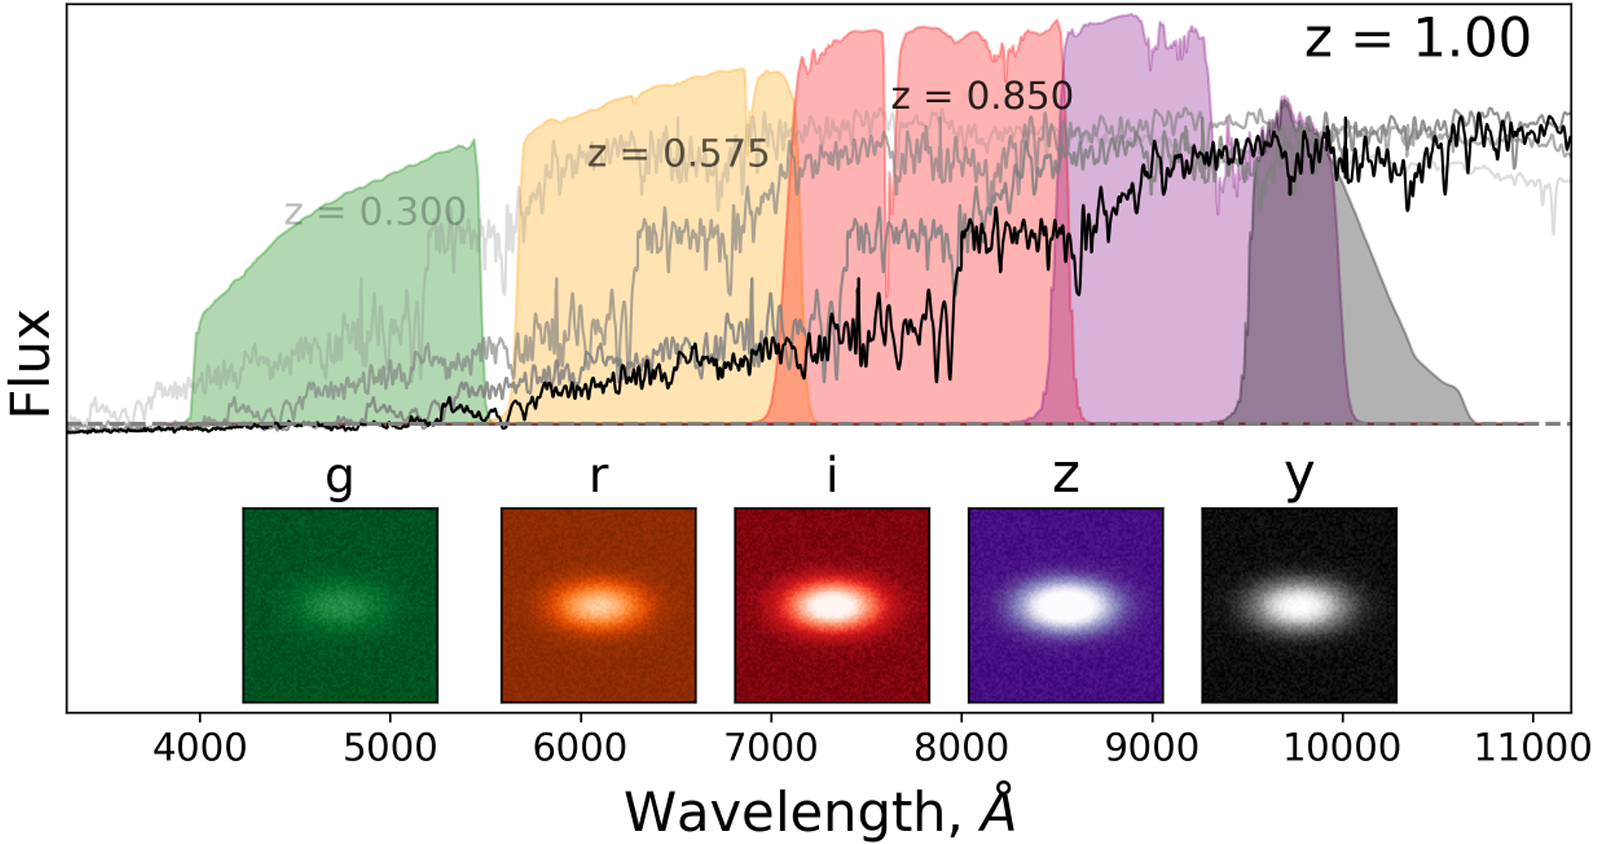
\includegraphics[width=0.80\textwidth]{figures/static_balmer.png}    
  }
  \caption{\label{fig:pz_redshift_basics}\small{A passive galaxy at
      different redshifts and how it will show up in various optical
      filters, giving us the ability to estimate its redshift and
      therefore distance. For many galaxies, the so-called
      'Balmer break' at 400 nm is a reliable feature that causes the
      flux to drop severely in bluer filters. Figure and caption
      by Jamie McCullough.}}
\end{figure*}

\begin{figure*}[ht]
  \centerline{
    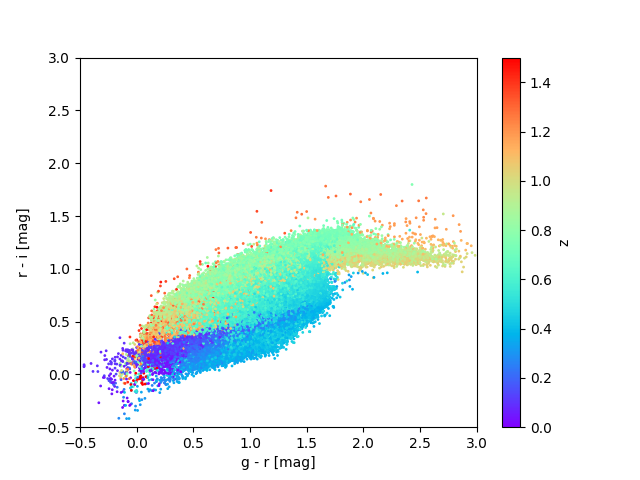
\includegraphics[width=0.45\textwidth]{figures/color_color_redshift_taskset_1_cardinal_10yr}    
    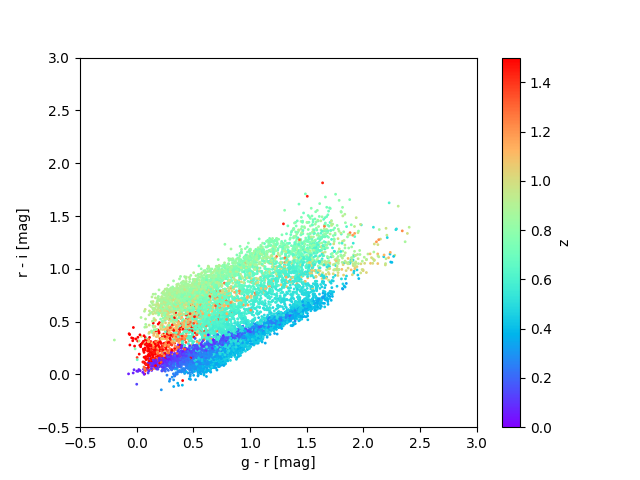
\includegraphics[width=0.45\textwidth]{figures/color_color_redshift_taskset_1_flagship_10yr}
  }
  \caption{\label{fig:color_color_redshift}\small{Redshifts plotted as
      a function of $r-i$ versus $g-r$ colors for a sample of objects
      in the cardinal (left) and flagship (right) simulations. These
      are plotted for the data for task set 1, i.e., for a sample of
      objects with $i < 23$.}}
\end{figure*}

This overly simple picture is complicated somewhat by the fact that
different galaxies have different intrinsic spectra and colors, as
seen in Fig.~\ref{fig:color_redshift}.

\begin{figure*}[ht]
  \centerline{
    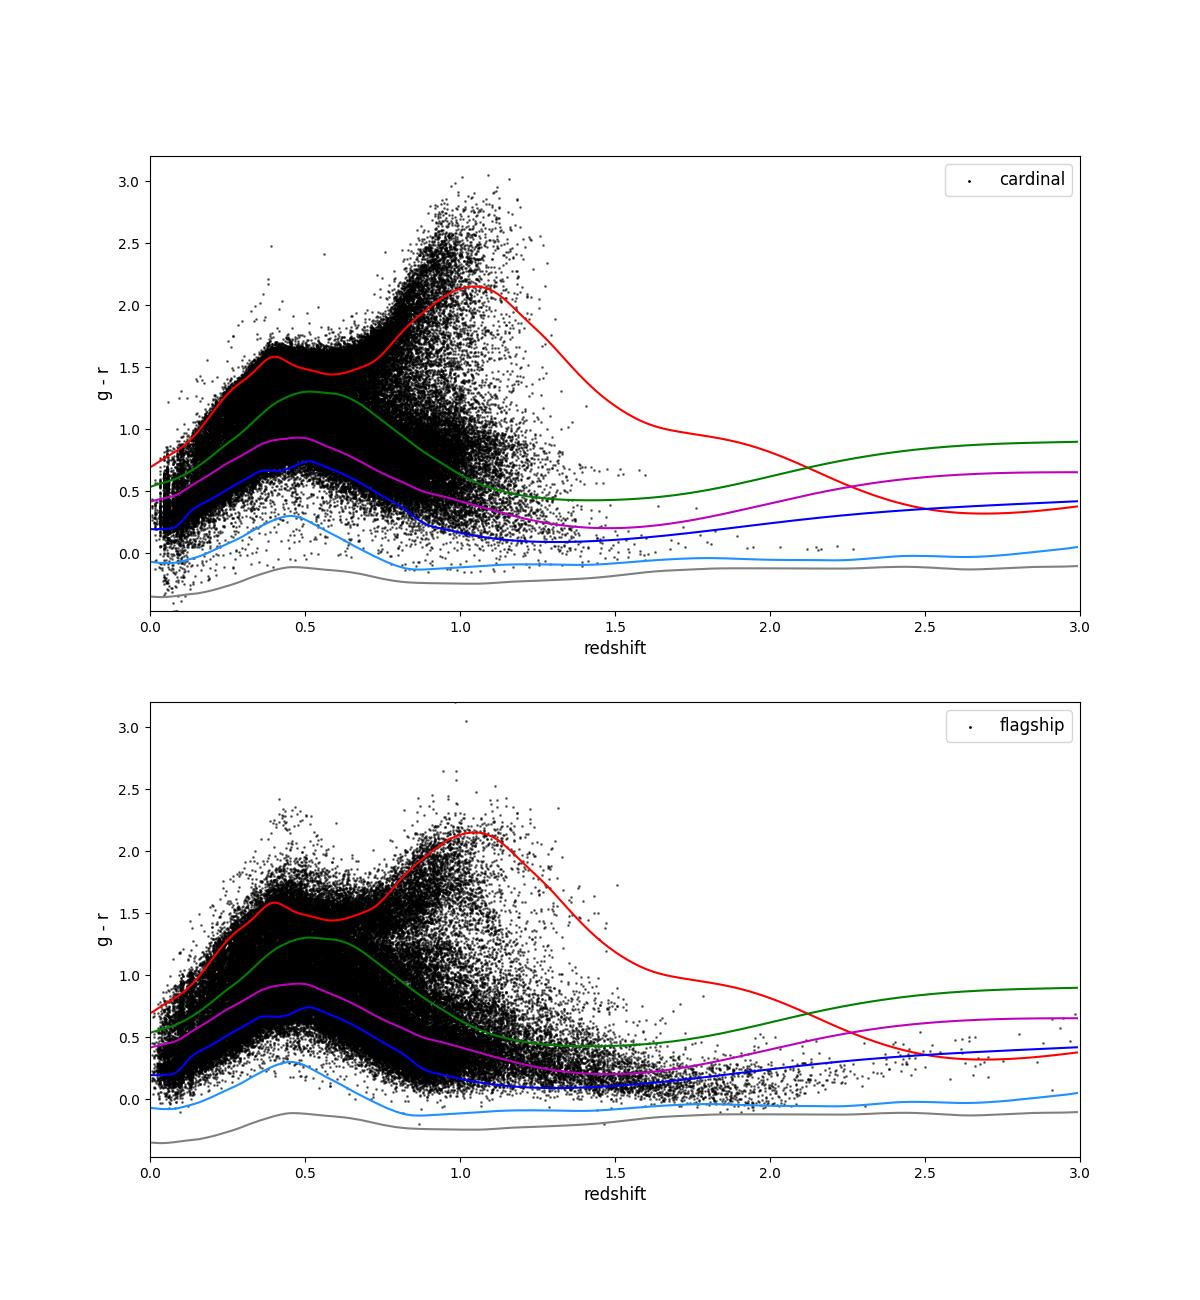
\includegraphics[width=0.80\textwidth]{figures/gr_vs_sz_sidebyside.jpg}    
  }
  \caption{\label{fig:color_redshift}\small{Color ($g-r$) plotted as a function of
      redshift for a sample of objects in the cardinal (top) and
      flagship (bottom) simulations. These are plotted for the data
      for task set 1, i.e., for a sample of objects with $i < 23$. The
      overlaid lines show the templates for several different types of galaxies.}}
\end{figure*}

This is further complicated by the fact that reference redshifts,
typically obtained by spectroscopy, slitless spectroscopy (i.e., GRISM
measurements), or narrowband photometric measurements, are not a
representative sample, as they are much easier to obtain for brighter
objects. Depending on the method used to obtain the reference
redshifts, they are also susceptible to errors such as confusing
different spectral lines or confusion of blended objects. Some of
the tasks in this data challenge encourage participants to try to
address these complications.
